\documentclass[11pt]{article}
\usepackage{classTools}
\usepackage[normalem]{ulem}

\begin{document}

\psHeader{7}{Wed Nov. 15, 2023 (11:59pm)}

\textbf{Your name: Cory Zimmerman}

\textbf{Collaborators: None}

\textbf{No. of late days used on previous psets: 0}

\textbf{No. of late days used after including this pset: 0}


The purpose of this problem set is to develop skills in implementing graph algorithms, appreciate the impact of different kinds of worst-case exponential algorithms in practice, and practice reducing problems to SAT.
\begin{enumerate}

    \item (Another coloring algorithm) 
  In the \href{https://github.com/Harvard-CS-120/cs120/tree/main/fall2023/psets/ps7}{Github repository for PS7}, we have given you basic data structures for graphs (in adjacency list representation) and colorings, an implementation of the coloring algorithm from ps5, and a variety of test cases (graphs) for coloring algorithms. For Windows users, use this \href{https://colab.research.google.com/drive/13nMhNMaDstVaEkxye61m8AV7nk9ks9uS#scrollTo=AbIalcylVVuu}{Google Colab} file to run your code.
  
  \begin{enumerate}
      
      \item Implement the reduction from 3-coloring to SAT given in class in the function \texttt{sat\_3\_coloring}, producing an input that can be fed into the SAT Solver \href{https://pysathq.github.io/usage/}{Glucose}, and verify its correctness by running \texttt{python3 -m ps7\_tests 3}. \label{part:SAT}
      \begin{quote}
          \color{purple}
          Done.
      \end{quote}

      \item Compare the efficiency of Exhaustive-Search 3-coloring, the $O(1.89^n)$-time BFS-based algorithm for 3-coloring from problem set 5 (feel free to use the staff solution or your own implementations from problem set 5), and your implementation from  Part~\ref{part:SAT} using \texttt{ps7\_experiments}. In the experiments file, we've provided code to generate two types of graphs (lines of rings and clusters of independent sets) and some new hard graph instances. For each of those types of graphs, how many of the given instances, if any, can each algorithm solve within 10 seconds (same time limit as problem set 5)? You should fill out the table and briefly discuss and try to explain your findings.

\begin{center}
\color{purple}
    \begin{tabular}{|c|l|l|l|}
    \hline 
    Algorithm
    & \multicolumn{1}{|p{2cm}|}{Exhaustive}
    & \multicolumn{1}{|p{2cm}|}{ISET BFS}
    & \multicolumn{1}{|p{2cm}|}{SAT Color}\\\hline
    \hline
        \# Solvable Ring Instances & 0 / 18 & 2 / 18 & 6 / 18 \\
        \# Solvable Cluster Instances  & 9 / 18 & 15 / 18 & 18 / 18 \\
        \# Solvable Hard Graphs  & 0 / 6 & 0 / 6 & 4 / 6 \\
        \hline
    \end{tabular}
    \vspace{1em}
  \begin{quote}
      \color{purple}
      It makes sense that the exhaustive algorithm underperformed ISET BFS and SAT for all trials. I found it interesting how thoroughly SAT crushed ISET BFS and how well it performed on the hard graphs. Considering asympototic behavior, ISET BFS is expected to run in $O(1.89^n)$ time, while the new algorithm reduces to SAT in $O(n + km)$ time. While 3-SAT, which this algorithm effectively uses, also doesn't have a polynomial runtime bound, it seems reasonable that an optimized SAT solver like PySAT wrapping well-tuned C and C++ code is able to handily outperform ISET BFS.
  \end{quote}
\end{center}

    \item (optional\footnote{This problem is meant to be done based on your enjoyment/interest and only if you have time. It won't make a difference between N, L, R-, and R grades, and course staff will deprioritize questions about this problem at office hours and on Ed.}) Find a graph $G$ such that Glucose takes more than 1 second to solve the SAT instance to which the 3-colorability of $G$ was reduced in part a, and $n$ is as small as you can make it. Describe your approach to finding such a $G$. 
  \end{enumerate}


\item (2SAT) Consider the following Boolean statements. 

\begin{enumerate}
    \item 
A:= ``Alice's grandparents got married."
\item B:= ``Alice was born."
\item C:=``Alice created a time machine in order to travel to the past."
\item D:=``Alice landed the time machine at her grandparents' first date and ruined it."
\end{enumerate}

Consider the CNF formula
$$(\neg A \vee B)\wedge (A \vee \neg B)\wedge (\neg B \vee C)\wedge (B \vee \neg C) \wedge (\neg C \vee D)\wedge ( C \vee \neg D) \wedge (\neg D \vee \neg A)\wedge (D \vee A).$$

If you interpret each clause above as an implication, are the implications reasonable? Explain briefly for 3 clauses of your choice. Draw the implication graph (for the whole formula, not just your chosen 3 clauses) and explain graphically why the CNF is unsatisfiable. 

\begin{quote}
    \color{purple}
    A logical clause of the form $(\neg \alpha \lor \beta)$ can be stated naturally as an implication of the form "if $\alpha$, then $\beta$". Expressing the terms of the CNF in this form makes them sound generally reasonable, assuming time travel is feasible and Alice has significant interest in her grandparents' first date: \\
    \begin{itemize}
        \item $\neg A \lor B$: "If Alice's grandparents got married, then Alice was born": I find this more likely than if her grandparents did not get married. 
        \item $B \lor \neg C$: "If Alice was not born, then Alice did not create a time machine in order to travel to the past". If Alice does not exist, she can't create a time machine, so I find this reasonable.
        \item $C \lor \neg D$: "If Alice did not create a time machine in order to travel to the past, then Alice did not land the time machine at her grandparents' first date and ruin it". I expect that Alice wouldn't have access to an available, pilotable time machine headed towards her grandparents' first date had she not created one, so, again, this makes sense to me.
    \end{itemize}

    \hspace{-7em}
    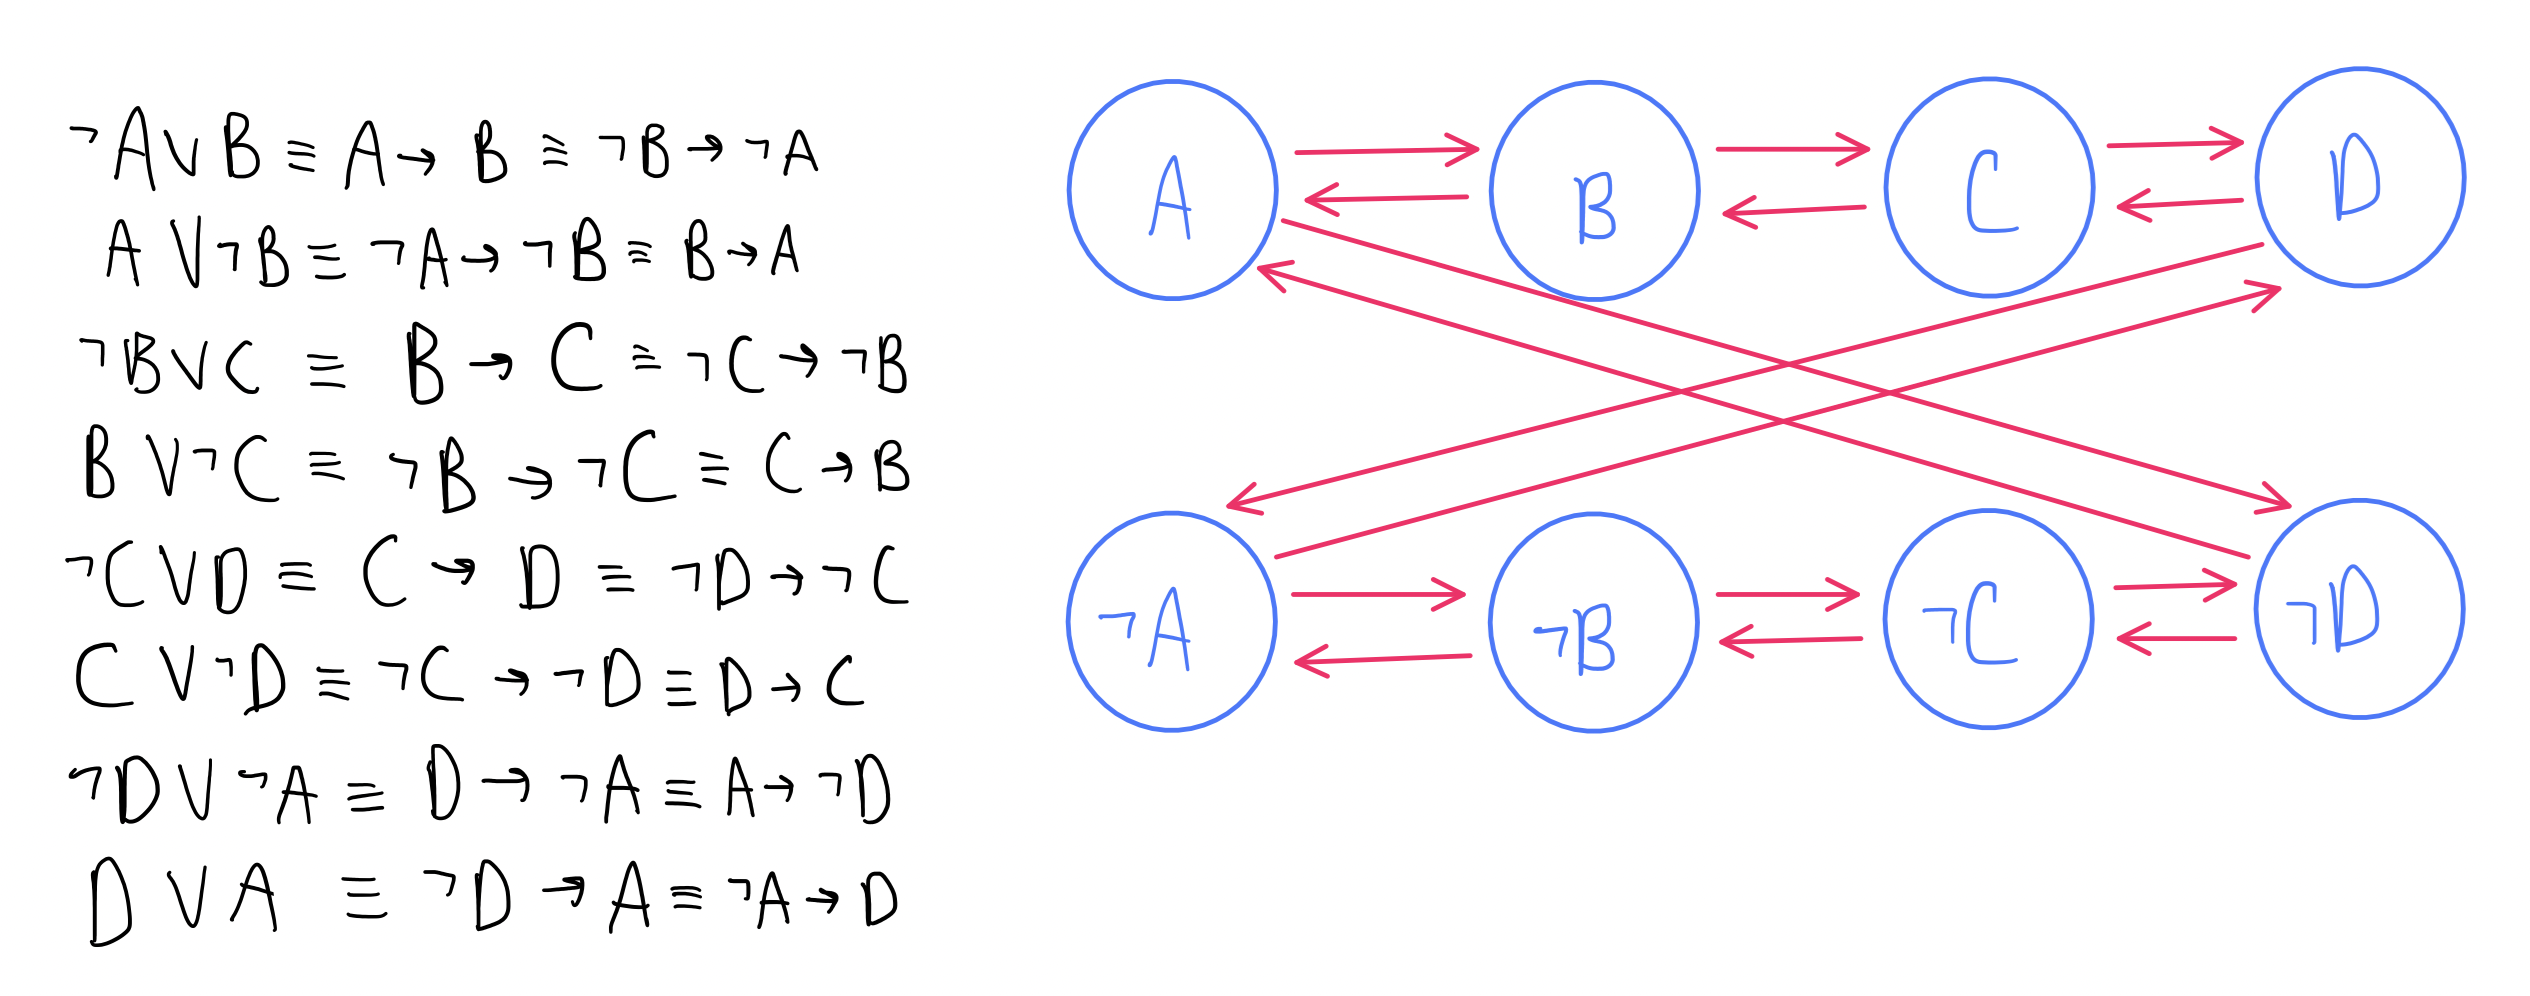
\includegraphics[scale=0.4]{implication_graph.png} \\

    By Theorem $3.3$ from the lecture notes, this CNF of width two is unsatisfiable because there exists a path from $A$ to $\neg D$ and from $\neg A$ to $D$ in the implication digraph. Stated more visually, because there's a visible loop in this graph of a width 2 CNF, it cannot be satisfiable. 
\end{quote}

\item (Reductions to SAT)  Consider the following problem.  From Harvard's $n$ CS concentrators (e.g. $n=400$), we want to form a team of exactly $k$ students (e.g. $k=30$) to represent Harvard in a new programming competition.  The programming competition problems may require expertise in any of $m$ different programming languages (e.g. $m=100$).  But each of the CS concentrators only knows a few different programming languages, with a different set per person. So we want to try to find $k$ Harvard CS concentrators such that between them, they know all $m$ languages. Formally, we want to solve the following computational problem:

\compprob{ProgrammingTeam()}
{A finite set $L=\{\ell_0,\ldots,\ell_{m-1}\}$ of programming languages; a finite set 
$S=\{s_0,\ldots,s_{n-1}\}$ of students; for each student $s\in S$, a set $K(s)\subseteq L$ of languages that student $s$ knows; and a team size $k\in \N$}
{A team $T\subseteq S$ of size $k$ that collectively knows all of the programming languages in $L$ (i.e. $\bigcup_{s\in T} K(s)=L$), if one exists}

\begin{enumerate}
    \item 
Show that ProgrammingTeam can be efficiently reduced to solving a SAT instance on $kn$ variables and $m+O(kn^2)$ clauses.  Prove the correctness of your reduction and analyze its runtime.

\begin{quote}
    \color{purple}
    I'll demonstrate this reduction by explaining how to algorithmically encode the inputs into a boolean formula that can be passed to SAT. First, however, recognize that, if $k$ ever exceeds $n$, we can immediately return $\bot$. This follows from the observation that we can never create a team of $k$ people from fewer than $k$ people. So, for the nontrivial parts of this reduction, $k \leq n$. In my reduction, I check this case, perform the encodings below, and then call SAT. If SAT returns $\bot$, my reduction also returns $\bot$. If SAT returns an assignment, my reduction extracts the student number from each assigned variable and returns those values in a set. With this in mind, consider how this reduction encodes inputs to SAT: \\
    
    Let $S_{i,j}$ express that student $i$ was selected for position $j$ on a team where $0 \leq i < n$ and $0 \leq j < k$. By the rules of combinatorics, this allows $kn$ variables in the boolean formula. Note: while the problem itself does not require ordered output, I'm introducing numerical order to the selected students in order to identifiy duplicates. \\

    My reduction to SAT requires encoding four aspects in the boolean formula: 
    \begin{enumerate}
        \item[1.] Every position on the team must be allocated.
        \item[2.] No student may be allocated for more than one position.
        \item[3.] No position may be allocated for more than one student.
        \item[4.] The members of the chosen team must collectively know every language.
    \end{enumerate}
    \vspace{1em}

    \textbf{Encoding (1)}: \\
    For every position, there must be at least one allocated student. This can be expressed in the following sequence: 
    $$(S_{0, 0} \lor S_{1, 0} \lor \dots \lor S_{n - 1, 0}) \lor \dots \lor (S_{0, k - 1} \lor S_{1, k - 1} \lor \dots \lor S_{n - 1, k - 1})$$
    In the sample above, the first clause verifies that at least one student is allocated to position $0$, and the final clause verifies that at least one student is allocated to position $k - 1$. With one clause for each position, there are $k$ of these in total. \\

    \textbf{Encoding (2)}: \\
    For every student, if they are assigned to position $j$, then they cannot be assigned to any position that is not $j$. Denote this as $j^c$. In implication form, this can be expressed as $S_{i, j} \implies \neg S_{i, j^c}$. Each implication can be expanded into $\neg S_{i, j} \lor \neg S_{i, j^c}$ to produce a formula like this: 
    $$(\neg S_{0, 0} \lor \neg S_{0, 1}) \land (\neg S_{0, 0} \lor \neg S_{0, 2}) \land \dots \land (\neg S_{0, 0} \lor \neg S_{0, k - 1}) \land \dots \land (\neg S_{0, k - 2} \lor \neg S_{0, k - 1})$$
    $$\dots$$
     $$(\neg S_{n - 1, 0} \lor \neg S_{n - 1, 1}) \land (\neg S_{n - 1, 0} \lor \neg S_{n - 1, 2}) \land \dots \land (\neg S_{n - 1, 0} \lor \neg S_{n - 1, k - 1}) \land \dots \land (\neg S_{n - 1, k - 2} \lor \neg S_{0, k - 1})$$
     In the sample above, the first three clauses encode "if student 0 is in position 0, then student 0 must not be in any other position". The final term implies checking every possible position that student $0$ may start in. The bottom row implies performing such verifications for every student. In total, this generates $O(k^2)$ clauses for $n$ students. However, because of the trivial case addressed at the beginning, it's guaranteed that $k \leq n$ such that the number of clauses needed for this encoding is bounded by $O(k \cdot n^2)$. \\

     \textbf{Encoding (3)}: \\
     For every position $i$, if student $j$ is assigned to that position, then no other student $i^c$ may be assigned there. In implication form, this is expressed as $S_{i, j} \implies S_{i^c, j}$ or equivalently as $\neg S_{i, j} \implies \neg S_{i^c, j}$. Encode this property like this: \\
    $$(\neg S_{0, 0} \lor \neg S_{1, 0}) \land (\neg S_{0, 0} \lor \neg S_{2, 0}) \land \dots \land (\neg S_{0, 0} \lor \neg S_{n - 1, 0})  \land \dots \land (\neg S_{n - 2, 0} \lor \neg S_{n - 1, 0})$$
    $$\dots$$
    $$(\neg S_{0, k - 1} \lor \neg S_{1, k - 1}) \land (\neg S_{0, k - 1} \lor \neg S_{2, k - 1}) \land \dots \land (\neg S_{0, k - 1} \lor \neg S_{n - 1, k - 1})  \land \dots \land (\neg S_{n - 2, k - 1} \lor \neg S_{n - 1, k - 1})$$
    In the sample above, the first three clauses encode "if position $0$ is allocated to student $0$, then position $0$ must not be allocated to any other student". The final term implies performing that check on every possible student who might be in position $0$. The bottom row implies performing such verifications for every position. In total, this generates $O(n^2)$ clauses for $k$  positions, yielding a clause count bounded by $O(kn^2)$. \\

    \textbf{Encoding (4)}: \\
    For every language, someone on the team must know it. Thus, for each of M languages, add a single clause to verify that at least one person in any position on the team knows the language. In the sample below, students $\alpha$ and $\beta$ are the only students who know language $m \in M$.
    $$(S_{\alpha, 0} \lor S_{\alpha, 1} \lor \dots \lor S_{\alpha, k - 1} \lor S_{\beta, 0} \lor S_{\beta, 1} \lor \dots \lor S_{\beta, k - 1})$$
    This produces one (potentially very long) clause verifying language inclusion in the selected group for every required language, so it adds $m$ clauses in total. \\

    \textbf{Input requirements}: \\
    Because the input variable, $S_{n, k}$ is bounded by $n \cdot k$ total combinations, this satisfies the variable requirement. Encoding the variants adds clauses of size $O(k) + O(kn^2) + O(kn^2) + O(m) = O(m + kn^2)$. Because of this, both input requirements are satisfied. \\

    \textbf{Correctness}: \\
    The algorithm accepts inputs $L$, $S$, and $K$ and uses these to encode a reduction to SAT. The boolean algorithm to SAT encodes the following properties: (1) the output team has $k$ members, (2 and 3) each of those members is uniquely assigned to the team, and (4) the members of the team collectively know every required language. By properly encoding these characteristics and returning the properly decoded results of an oracle call to SAT, my program produces a valid output to ProgrammingTeam for every valid input, making it a correct algorithm. \\

    \textbf{Runtime}: \\
    The runtime of this reduction is dominated by performing the encodings. Consider each. Encoding (1) can be performed in a loop iterating "for each of $k$ positions, for each of $n$ students" and has runtime $O(kn)$. Encoding (2) loops "for each of $n$ students, for each of $k$ positions, for each of $k$ positions". As established earlier, $k \leq n$ such that this runtime can be bounded by $O(kn^2)$. Encoding (3) loops "for each of $k$ positions, for each of $n$ students, for each of $n$ students", which completes in time $O(kn^2)$. And Encoding (4) loops "for each of $m$ languages, for each of $n$ students, for each of $k$ positions", which runs in time $O(mnk)$. Finally, decoding the result of SAT into a set will take at most the number of results in a satisfying assignment, $O(k)$. Thus, the runtime of my reduction completes in time $O(kn + kn^2 + kn^2 + mnk + k)$, which can be simplified into $O(kn^2 + mnk)$.
    
    
\end{quote}

\item 
(optional\footnotemark[1])
Come up with a more efficient reduction that produces a SAT instance with $O(kn)$ variables and $m+O(kn)$ clauses (or even $m+O(n\log k)$ clauses). (Hint: something like $\psi_{n,k}$ or $\tau_\ell$ formulas from the Section 7 problem on IndependentSet$\leq$ SAT might be useful.)
\end{enumerate}

 \item Please fill out the Problem Set 7 Feedback Survey here: \href{https://forms.gle/bNfaHbXutBiXq97v6}{https://forms.gle/bNfaHbXutBiXq97v6}. We appreciate your feedback!

\end{enumerate}



\end{document}
